\section{Übergeordnete Module}
\label{sec:knf:module}

Die acht grundlegenden Module aus den vorhergehenden Abschnitten werden in diesem Abschnitt genutzt,
um hierarchisch die vollständige Kompressionsfunktion von \glos{sha256} zu erzeugen. Eine einfache Lösung wäre es,
jeweils ein Modul für die Rundenfunktion und für die Erweiterung der Eingabe zu Erstellen. Diese werden
im Modul für die Kompressionsfunktion dann 64 bzw. 48 mal eingebunden. Das löst zwar die Generierung der konjunktiven
Normalform, ist jedoch für eine Analyse unter Umständen zu grob. Sollte es gelingen, Wissen mit CryptoMiniSat zu erwerben,
und einzelnen Modulen zuzuordnen, müsste eine weitere Zuordnung innerhalb des Moduls per Hand erfolgen.

Um dieses Problem zu vermeiden, werden zunächst kleinere Module definiert. Abbildung \ref{fig:sha256M} zeigt auf der linken
Seite zwei Module die Bestandteil der Rundenfunktion sind und jeweils aus drei anderen Modulen bestehen. Interessant ist dabei,
dass A und E jeweils Eingang in zwei Module finden, deren Ergebnisse durch eine Addition wieder zusammengeführt werden. Die
Analyse dieser Rekonvergenzen ist besonders interessant und wird durch die beiden Module vereinfacht.
\begin{figure}[!h]
  \centering
  \begin{minipage}[l]{9.5cm}
    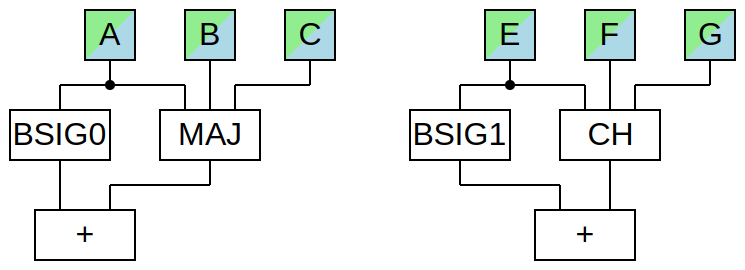
\includegraphics[scale=0.4]{images/sha256coreM}
  \end{minipage}
  \begin{minipage}[l]{3cm}
    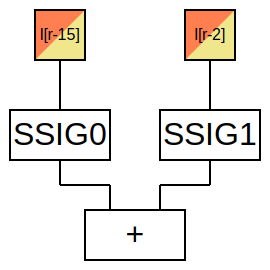
\includegraphics[scale=0.4]{images/sha256prepM}
  \end{minipage}    
  \caption{Erweiterte Module von \glos{sha256}}
  \label{fig:sha256M}
\end{figure}

Ein weiteres Modul ist Bestandteil der Erweiterung der Eingabe und in Abbildung \ref{fig:sha256M} auf der rechten Seite
dargestellt. Bei der Erweiterung der Eingabe werden vier Werte Addiert, wobei zwei davon zunächst durch die $ \sigma $-Funktionen
transformiert werden. Da es keine Rolle spielt, in welcher Reihenfolge die Addition durchgeführt wird, werden diese
beiden zunächst in einem eigenen Modul addiert. Da jedes Eingabebit der $ \sigma $-Funktionen Einfluss auf bis zu
drei Ausgabebits hat, könnten sich möglicherweise Rückschlüsse auf die jeweils anderen Eingabebits ziehen lassen.
Mit Hilfe dieses Moduls und weiteren Additionen, wird schließlich ein Modul für die vollständige Erweiterung der Eingabe
(siehe Abbildung \ref{fig:sha256prep}) erstellt. Die verbleibenden beiden Werte werden zunächst Addiert, um das Ergebnis
dann mit dem Ergebnis des Moduls zu addieren.

Die beiden erstgenannten Module werden ebenfalls zusammen mit weiteren Additionen genutzt, um ein Modul für die vollständige
Rundenfunktion (siehe Abbildung \ref{fig:sha256core}) zu realisieren. Außen vor bleibt dabei die Addition der Konstante.
Dadurch kann erworbenes Wissen auf alle 64 Runden angewendet werden, da es sich jedes Mal um das gleiche Modul handelt.
In einem weiteren Modul wird schließlich die Rundenfunktion mit der Addition der Konstante zusammengeführt.
Erworbenes Wissen, was auf der Konstante basiert, kann dadurch in diesem Modul gesammelt werden, falls es sich in einem
zweiten Schritt als allgemeingültig erweist.

Abschließend werden die genannten Module in einem Modul für die vollständige Rundenfunktion genutzt. Zusätzlich erfolgt in
diesem Modul auch die \ref{fig:sha256single} Addtion \TODO{erledigen}

Erweiterungsfunktion\\
Rundenfunktion\\
Rundenfunktion + Konstante\\
\glos{sha256} als ganzes: wissen hinzufügen und mehrfache verwendung bei bitcoin\\
~\\
Rekonvergenzen bei ersten beiden finden.\\
~\\
baum\\
hierarchie durch level:\\
subaddierer bekommen ihre ebene: 1 bis 4\\
module aus grafik ebene 10\\
11\\
20\\
21\\
sha als ganzes: 30\\
~\\
betrachtung der erweiterung als teil der runden 17 bis 64